\begin{frame}
	\myheading{Module 11.1 : The convolution operation}
\end{frame}

%%%%%%%%%%%%%%%%%%%%%%%%%%%%%%%%%%%%%%%%%%%%%%%%%%%%%%%%%%%%%%%%%%%%%%%%%%%%%%

\begin{frame}
    \begin{columns}
        \column{0.5\textwidth}<1->
        \begin{overlayarea}{\textwidth}{\textheight}
                \vspace{3mm}
            
                \onslide<1->{\begin{minipage}[t]{0.25\textwidth}
                \includegraphics[width=\textwidth]{images/spaceship.jpg}
                \end{minipage}}
                \onslide<2->{\begin{minipage}[t]{0.25\textwidth}
                \includegraphics[width=\textwidth]{images/spaceship.jpg}
                \end{minipage}}
                \onslide<3->{\begin{minipage}[t]{0.25\textwidth}
                \includegraphics[width=\textwidth]{images/spaceship.jpg}
                \end{minipage}}
                
                \onslide<1->{\begin{minipage}[t]{0.25\textwidth}
                \hspace{4mm}$x_0$
                \end{minipage}}
                \onslide<2->{\begin{minipage}[t]{0.25\textwidth}
                \hspace{4mm}$x_1$
                \end{minipage}}
                \onslide<3->{\begin{minipage}[t]{0.25\textwidth}
                \hspace{4mm}$x_2$
                \end{minipage}}
                \hspace{3mm}
                \onslide<7-9>{\begin{minipage}[t]{0.25\textwidth}
                \begin{equation*}
                    s_t= \onslide<7->{\sum_{a=0}^{\infty}x_{t-a}\tikzmark{xa} w_{-a}\tikzmark{ab}} = \onslide<8->{(\tikzmark{x}x \tikzmark{star}\ast \tikzmark{w}w)_t\tikzmark{cd}}
                \end{equation*}
                \onslide<9->{
                		\begin{tikzpicture}[overlay,remember picture]
	\node (xt) [below of = xa, node distance = 3 em, anchor=west]{\footnotesize \textsf{input}};
	\draw[<-, in=90, out=-90] (x.south)++(.25em,-.5ex) to (xt.north);
	
	\node (start) [below of = ab, node distance = 4 em, anchor=west] {\footnotesize \textsf{convolution}};
	\draw[<-, in=90, out=-90] (star.south)++(.25em,-.5ex) to (start.north);
	
	\node (wt) [below of = cd, node distance = 3 em, anchor=west] {\footnotesize \textsf{filter}};
	\draw[<-, in=90, out=-90] (w.south)++(.25em,-.5ex) to (wt.north);

\end{tikzpicture}

                \end{minipage}
                }}
        \end{overlayarea}
        
        \column{0.5\textwidth}<1->
        \begin{overlayarea}{\textwidth}{\textheight}
            \begin{itemize}
                \justifying
                \item<1-> Suppose we are tracking the position of an aeroplane using a laser sensor at discrete time intervals
                \item<4-> Now suppose our sensor is noisy
                \item<5-> To obtain a less noisy estimate we would like to average several measurements
                \item<6-> More recent measurements are more important so we would like to take a weighted average
            \end{itemize}
        \end{overlayarea}
    \end{columns}
\end{frame}

%%%%%%%%%%%%%%%%%%%%%%%%%%%%%%%%%%%%%%%%%%%%%%%%%%%%%%%%%%%%%%%%%%%%%%%%%%%%%%

\begin{frame}
	\begin{columns}
		\column{0.5\textwidth}<1->
		\begin{overlayarea}{\textwidth}{\textheight}
			\begin{minipage}[t]{0.25\textwidth}
				\onslide<1->{
					\begin{equation*}
						s_t=\sum_{a=0}^{6}x_{t-a} w_{-a}
					\end{equation*}
				}
				\vspace{1cm}
			\end{minipage}
			           
			\begin{minipage}[t]{0.25\textwidth}
				           
				
				\only<3>{
					\begin{table}[h]
						%\small
						\renewcommand{\arraystretch}{1.5}
						\renewcommand{\tabcolsep}{1mm}
						\resizebox{4.6\textwidth}{!}{%
							\begin{tabular}{p{0.1cm}p{0.1cm}p{0.1cm}p{0.1cm}p{0.1cm}p{0.1cm}p{0.1cm}p{0.1cm}p{0.1cm}p{0.1cm}p{0.1cm}p{0.1cm}p{0.1cm}p{0.1cm}}
								                  
								                     &                       & $w_{-6}$                  & $w_{-5}$                  & $w_{-4}$                  & $w_{-3}$                  & $w_{-2}$                  & $w_{-1}$                                         & $w_{0}$                                          &                                                  &                                                  &                                                  &                                                  &                                                  \\ \cline{8-9}
								\cline{3-9}
								W                    & \multicolumn{1}{l|}{} & \multicolumn{1}{c|}{0.01} & \multicolumn{1}{c|}{0.01} & \multicolumn{1}{c|}{0.02} & \multicolumn{1}{c|}{0.02} & \multicolumn{1}{c|}{0.04} & \multicolumn{1}{c|}{0.4}                         & \multicolumn{1}{c|}{0.5}                         &                                                  &                                                  &                                                  &                                                  &                                                  \\ \cline{3-9}
								\multicolumn{1}{l}{} &                       & \multicolumn{1}{l}{}      & \multicolumn{1}{l}{}      & \multicolumn{1}{l}{}      & \multicolumn{1}{l}{}      & \multicolumn{1}{l}{}      & \multicolumn{1}{l}{}                             & \multicolumn{1}{l}{}                             & \multicolumn{1}{l}{}                             &                                                  &                                                  &                                                  &                                                  \\ \cline{3-14} 
								X                    & \multicolumn{1}{l|}{} & \multicolumn{1}{c|}{1.00} & \multicolumn{1}{c|}{1.10} & \multicolumn{1}{c|}{1.20} & \multicolumn{1}{c|}{1.40} & \multicolumn{1}{c|}{1.70} & \multicolumn{1}{c|}{1.80}                        & \multicolumn{1}{c|}{1.90}                        & \multicolumn{1}{c|}{2.10}                        & \multicolumn{1}{c|}{2.20}                        & \multicolumn{1}{c|}{2.40}                        & \multicolumn{1}{c|}{2.50}                        & \multicolumn{1}{c|}{2.70}                        \\ \cline{3-14} 
								\multicolumn{1}{l}{} &                       & \multicolumn{1}{l}{}      & \multicolumn{1}{l}{}      & \multicolumn{1}{l}{}      & \multicolumn{1}{l}{}      & \multicolumn{1}{l}{}      & \multicolumn{1}{l}{}                             & \multicolumn{1}{l}{}                             & \multicolumn{1}{l}{}                             &                                                  &                                                  &                                                  &                                                  \\  \cline{9-14} 
								S                    &                       &                           &                           &                           &                           &                           & \multicolumn{1}{c|}{{\color[HTML]{FFFFFF} 0.00}} & \multicolumn{1}{c|}{{\color[HTML]{333333} 1.80}} & \multicolumn{1}{c|}{{\color[HTML]{FFFFFF} 0.00}} & \multicolumn{1}{c|}{{\color[HTML]{FFFFFF} 0.00}} & \multicolumn{1}{c|}{{\color[HTML]{FFFFFF} 0.00}} & \multicolumn{1}{c|}{{\color[HTML]{FFFFFF} 0.00}} & \multicolumn{1}{c|}{{\color[HTML]{FFFFFF} 0.00}} \\ \cline{9-14} 
							\end{tabular}
						}
					\end{table}
					
				}
				           
				\only<4>{
					\begin{table}[h]
						%\scriptsize
						\renewcommand{\arraystretch}{1.5}
						\renewcommand{\tabcolsep}{1mm}
						\resizebox{4.6\textwidth}{!}{%
							\begin{tabular}{p{0.1cm}p{0.1cm}p{0.1cm}p{0.1cm}p{0.1cm}p{0.1cm}p{0.1cm}p{0.1cm}p{0.1cm}p{0.1cm}p{0.1cm}p{0.1cm}p{0.1cm}p{0.1cm}}
								                  
								                     &                       &                           & $w_{-6}$                  & $w_{-5}$                  & $w_{-4}$                  & $w_{-3}$                  & $w_{-2}$                                         & $w_{-1}$                                         & $w_{0}$                                          &                                                  &                                                  &                                                  &                                                  \\ \cline{8-10}
								\cline{4-10}
								W                    &                       & \multicolumn{1}{c|}{}     & \multicolumn{1}{c|}{0.01} & \multicolumn{1}{c|}{0.01} & \multicolumn{1}{c|}{0.02} & \multicolumn{1}{c|}{0.02} & \multicolumn{1}{c|}{0.04}                        & \multicolumn{1}{c|}{0.4}                         & \multicolumn{1}{c|}{0.5}                         &                                                  &                                                  &                                                  &                                                  \\ \cline{4-10}
								\multicolumn{1}{l}{} &                       & \multicolumn{1}{l}{}      & \multicolumn{1}{l}{}      & \multicolumn{1}{l}{}      & \multicolumn{1}{l}{}      & \multicolumn{1}{l}{}      & \multicolumn{1}{l}{}                             & \multicolumn{1}{l}{}                             & \multicolumn{1}{l}{}                             &                                                  &                                                  &                                                  &                                                  \\ \cline{3-14} 
								X                    & \multicolumn{1}{l|}{} & \multicolumn{1}{c|}{1.00} & \multicolumn{1}{c|}{1.10} & \multicolumn{1}{c|}{1.20} & \multicolumn{1}{c|}{1.40} & \multicolumn{1}{c|}{1.70} & \multicolumn{1}{c|}{1.80}                        & \multicolumn{1}{c|}{1.90}                        & \multicolumn{1}{c|}{2.10}                        & \multicolumn{1}{c|}{2.20}                        & \multicolumn{1}{c|}{2.40}                        & \multicolumn{1}{c|}{2.50}                        & \multicolumn{1}{c|}{2.70}                        \\ \cline{3-14} 
								\multicolumn{1}{l}{} &                       & \multicolumn{1}{l}{}      & \multicolumn{1}{l}{}      & \multicolumn{1}{l}{}      & \multicolumn{1}{l}{}      & \multicolumn{1}{l}{}      & \multicolumn{1}{l}{}                             & \multicolumn{1}{l}{}                             & \multicolumn{1}{l}{}                             &                                                  &                                                  &                                                  &                                                  \\  \cline{9-14} 
								S                    &                       &                           &                           &                           &                           &                           & \multicolumn{1}{c|}{{\color[HTML]{FFFFFF} 0.00}} & \multicolumn{1}{c|}{{\color[HTML]{333333} 1.80}} & \multicolumn{1}{c|}{{\color[HTML]{333333} 1.96}} & \multicolumn{1}{c|}{{\color[HTML]{FFFFFF} 0.00}} & \multicolumn{1}{c|}{{\color[HTML]{FFFFFF} 0.00}} & \multicolumn{1}{c|}{{\color[HTML]{FFFFFF} 0.00}} & \multicolumn{1}{c|}{{\color[HTML]{FFFFFF} 0.00}} \\ \cline{9-14} 
							\end{tabular}
						}
					\end{table}
				}
				\only<5>{
					\begin{table}[h]
						%\scriptsize
						\renewcommand{\arraystretch}{1.5}
						\renewcommand{\tabcolsep}{1mm}
						\resizebox{4.6\textwidth}{!}{%
							\begin{tabular}{p{0.1cm}p{0.1cm}p{0.1cm}p{0.1cm}p{0.1cm}p{0.1cm}p{0.1cm}p{0.1cm}p{0.1cm}p{0.1cm}p{0.1cm}p{0.1cm}p{0.1cm}p{0.1cm}}
								                  
								                     &                       &                           &                           & $w_{-6}$                  & $w_{-5}$                  & $w_{-4}$                  & $w_{-3}$                                         & $w_{-2}$                                         & $w_{-1}$                                         & $w_{0}$                                          &                                                  &                                                  &                                                  \\ \cline{8-11}
								\cline{5-11}
								W                    &                       &                           & \multicolumn{1}{c|}{}     & \multicolumn{1}{c|}{0.01} & \multicolumn{1}{c|}{0.01} & \multicolumn{1}{c|}{0.02} & \multicolumn{1}{c|}{0.02}                        & \multicolumn{1}{c|}{0.04}                        & \multicolumn{1}{c|}{0.4}                         & \multicolumn{1}{l|}{0.5}                         &                                                  &                                                  &                                                  \\ \cline{5-11}
								\multicolumn{1}{l}{} &                       & \multicolumn{1}{l}{}      & \multicolumn{1}{l}{}      & \multicolumn{1}{l}{}      & \multicolumn{1}{l}{}      & \multicolumn{1}{l}{}      & \multicolumn{1}{l}{}                             & \multicolumn{1}{l}{}                             & \multicolumn{1}{l}{}                             &                                                  &                                                  &                                                  &                                                  \\ \cline{3-14} 
								X                    & \multicolumn{1}{l|}{} & \multicolumn{1}{c|}{1.00} & \multicolumn{1}{c|}{1.10} & \multicolumn{1}{c|}{1.20} & \multicolumn{1}{c|}{1.40} & \multicolumn{1}{c|}{1.70} & \multicolumn{1}{c|}{1.80}                        & \multicolumn{1}{c|}{1.90}                        & \multicolumn{1}{c|}{2.10}                        & \multicolumn{1}{c|}{2.20}                        & \multicolumn{1}{c|}{2.40}                        & \multicolumn{1}{c|}{2.50}                        & \multicolumn{1}{c|}{2.70}                        \\ \cline{3-14} 
								\multicolumn{1}{l}{} &                       & \multicolumn{1}{l}{}      & \multicolumn{1}{l}{}      & \multicolumn{1}{l}{}      & \multicolumn{1}{l}{}      & \multicolumn{1}{l}{}      & \multicolumn{1}{l}{}                             & \multicolumn{1}{l}{}                             & \multicolumn{1}{l}{}                             &                                                  &                                                  &                                                  &                                                  \\  \cline{9-14} 
								S                    &                       &                           &                           &                           &                           &                           & \multicolumn{1}{c|}{{\color[HTML]{FFFFFF} 0.00}} & \multicolumn{1}{c|}{{\color[HTML]{333333} 1.80}} & \multicolumn{1}{c|}{{\color[HTML]{333333} 1.96}} & \multicolumn{1}{c|}{{\color[HTML]{333333} 2.11}} & \multicolumn{1}{c|}{{\color[HTML]{FFFFFF} 0.00}} & \multicolumn{1}{c|}{{\color[HTML]{FFFFFF} 0.00}} & \multicolumn{1}{c|}{{\color[HTML]{FFFFFF} 0.00}} \\ \cline{9-14} 
							\end{tabular}
						}
					\end{table}
				}
				\only<6>{
					\begin{table}[h]
						%\scriptsize
						\renewcommand{\arraystretch}{1.5}
						\renewcommand{\tabcolsep}{1mm}
						\resizebox{4.6\textwidth}{!}{%
							\begin{tabular}{p{0.1cm}p{0.1cm}p{0.1cm}p{0.1cm}p{0.1cm}p{0.1cm}p{0.1cm}p{0.1cm}p{0.1cm}p{0.1cm}p{0.1cm}p{0.1cm}p{0.1cm}p{0.1cm}}
								                  
								                     &                       &                           &                           &                           & $w_{-6}$                  & $w_{-5}$                  & $w_{-4}$                                         & $w_{-3}$                                         & $w_{-2}$                                         & $w_{-1}$                                         & $w_{0}$                                          &                                                  &                                                  \\ \cline{8-12}
								\cline{6-12}
								W                    &                       &                           &                           & \multicolumn{1}{c|}{}     & \multicolumn{1}{c|}{0.01} & \multicolumn{1}{c|}{0.01} & \multicolumn{1}{c|}{0.02}                        & \multicolumn{1}{c|}{0.02}                        & \multicolumn{1}{c|}{0.04}                        & \multicolumn{1}{l|}{0.4}                         & \multicolumn{1}{l|}{0.5}                         &                                                  &                                                  \\ \cline{6-12}
								\multicolumn{1}{l}{} &                       & \multicolumn{1}{l}{}      & \multicolumn{1}{l}{}      & \multicolumn{1}{l}{}      & \multicolumn{1}{l}{}      & \multicolumn{1}{l}{}      & \multicolumn{1}{l}{}                             & \multicolumn{1}{l}{}                             & \multicolumn{1}{l}{}                             &                                                  &                                                  &                                                  &                                                  \\ \cline{3-14} 
								X                    & \multicolumn{1}{l|}{} & \multicolumn{1}{c|}{1.00} & \multicolumn{1}{c|}{1.10} & \multicolumn{1}{c|}{1.20} & \multicolumn{1}{c|}{1.40} & \multicolumn{1}{c|}{1.70} & \multicolumn{1}{c|}{1.80}                        & \multicolumn{1}{c|}{1.90}                        & \multicolumn{1}{c|}{2.10}                        & \multicolumn{1}{c|}{2.20}                        & \multicolumn{1}{c|}{2.40}                        & \multicolumn{1}{c|}{2.50}                        & \multicolumn{1}{c|}{2.70}                        \\ \cline{3-14} 
								\multicolumn{1}{l}{} &                       & \multicolumn{1}{l}{}      & \multicolumn{1}{l}{}      & \multicolumn{1}{l}{}      & \multicolumn{1}{l}{}      & \multicolumn{1}{l}{}      & \multicolumn{1}{l}{}                             & \multicolumn{1}{l}{}                             & \multicolumn{1}{l}{}                             &                                                  &                                                  &                                                  &                                                  \\  \cline{9-14} 
								S                    &                       &                           &                           &                           &                           &                           & \multicolumn{1}{c|}{{\color[HTML]{FFFFFF} 0.00}} & \multicolumn{1}{c|}{{\color[HTML]{333333} 1.80}} & \multicolumn{1}{c|}{{\color[HTML]{333333} 1.96}} & \multicolumn{1}{c|}{{\color[HTML]{333333} 2.11}} & \multicolumn{1}{c|}{{\color[HTML]{333333} 2.16}} & \multicolumn{1}{c|}{{\color[HTML]{FFFFFF} 0.00}} & \multicolumn{1}{c|}{{\color[HTML]{FFFFFF} 0.00}} \\ \cline{9-14} 
							\end{tabular}
						}
					\end{table}
				}
				\only<7>{
					\begin{table}[h]
						%\scriptsize
						\renewcommand{\arraystretch}{1.5}
						\renewcommand{\tabcolsep}{1mm}
						\resizebox{4.6\textwidth}{!}{%
							\begin{tabular}{p{0.1cm}p{0.1cm}p{0.1cm}p{0.1cm}p{0.1cm}p{0.1cm}p{0.1cm}p{0.1cm}p{0.1cm}p{0.1cm}p{0.1cm}p{0.1cm}p{0.1cm}p{0.1cm}}
								                  
								                     &                       &                           &                           &                           &                           & $w_{-6}$                  & $w_{-5}$                                         & $w_{-4}$                                         & $w_{-3}$                                         & $w_{-2}$                                         & $w_{-1}$                                         & $w_{0}$                                          &                                                  \\ \cline{8-13}
								\cline{7-13}
								W                    &                       &                           &                           &                           & \multicolumn{1}{c|}{}     & \multicolumn{1}{c|}{0.01} & \multicolumn{1}{c|}{0.01}                        & \multicolumn{1}{c|}{0.02}                        & \multicolumn{1}{c|}{0.02}                        & \multicolumn{1}{c|}{0.04}                        & \multicolumn{1}{c|}{0.4}                         & \multicolumn{1}{c|}{0.5}                         &                                                  \\ \cline{7-13}
								\multicolumn{1}{l}{} &                       & \multicolumn{1}{l}{}      & \multicolumn{1}{l}{}      & \multicolumn{1}{l}{}      & \multicolumn{1}{l}{}      & \multicolumn{1}{l}{}      & \multicolumn{1}{l}{}                             & \multicolumn{1}{l}{}                             & \multicolumn{1}{l}{}                             & \multicolumn{1}{l}{}                             & \multicolumn{1}{l}{}                             & \multicolumn{1}{l}{}                             &                                                  \\ \cline{3-14} 
								X                    & \multicolumn{1}{l|}{} & \multicolumn{1}{c|}{1.00} & \multicolumn{1}{c|}{1.10} & \multicolumn{1}{c|}{1.20} & \multicolumn{1}{c|}{1.40} & \multicolumn{1}{c|}{1.70} & \multicolumn{1}{c|}{1.80}                        & \multicolumn{1}{c|}{1.90}                        & \multicolumn{1}{c|}{2.10}                        & \multicolumn{1}{c|}{2.20}                        & \multicolumn{1}{c|}{2.40}                        & \multicolumn{1}{c|}{2.50}                        & \multicolumn{1}{c|}{2.70}                        \\ \cline{3-14} 
								\multicolumn{1}{l}{} &                       & \multicolumn{1}{l}{}      & \multicolumn{1}{l}{}      & \multicolumn{1}{l}{}      & \multicolumn{1}{l}{}      & \multicolumn{1}{l}{}      & \multicolumn{1}{l}{}                             & \multicolumn{1}{l}{}                             & \multicolumn{1}{l}{}                             & \multicolumn{1}{l}{}                             & \multicolumn{1}{l}{}                             & \multicolumn{1}{l}{}                             &                                                  \\  \cline{9-14} 
								S                    &                       &                           &                           &                           &                           &                           & \multicolumn{1}{c|}{{\color[HTML]{FFFFFF} 0.00}} & \multicolumn{1}{c|}{{\color[HTML]{333333} 1.80}} & \multicolumn{1}{c|}{{\color[HTML]{333333} 1.96}} & \multicolumn{1}{c|}{{\color[HTML]{333333} 2.11}} & \multicolumn{1}{c|}{{\color[HTML]{333333} 2.16}} & \multicolumn{1}{c|}{{\color[HTML]{333333} 2.28}} & \multicolumn{1}{c|}{{\color[HTML]{FFFFFF} 0.00}} \\ \cline{9-14} 
								
							\end{tabular}
						}
					\end{table}
				}
				
				\only<8->{
					\begin{table}[h]
						%\scriptsize
						\renewcommand{\arraystretch}{1.5}
						\renewcommand{\tabcolsep}{1mm}
						\resizebox{4.6\textwidth}{!}{%
							\begin{tabular}{p{0.1cm}p{0.1cm}p{0.1cm}p{0.1cm}p{0.1cm}p{0.1cm}p{0.1cm}p{0.1cm}p{0.1cm}p{0.1cm}p{0.1cm}p{0.1cm}p{0.1cm}p{0.1cm}}
								                     &                       &                           &                           &                           &                           &                           & $w_{-6}$                                         & $w_{-5}$                                         & $w_{-4}$                                         & $w_{-3}$                                         & $w_{-2}$                                         & $w_{-1}$                                         & $w_{0}$                                           \\ \cline{8-14}
								\cline{8-14}
								W                    &                       &                           &                           &                           &                           & \multicolumn{1}{c|}{}     & \multicolumn{1}{c|}{0.01}                        & \multicolumn{1}{c|}{0.01}                        & \multicolumn{1}{c|}{0.02}                        & \multicolumn{1}{c|}{0.02}                        & \multicolumn{1}{c|}{0.04}                           & \multicolumn{1}{c|}{0.4}                         & \multicolumn{1}{l|}{0.5}                          \\ \cline{8-14} 
								\multicolumn{1}{l}{} &                       & \multicolumn{1}{l}{}      & \multicolumn{1}{l}{}      & \multicolumn{1}{l}{}      & \multicolumn{1}{l}{}      & \multicolumn{1}{l}{}      & \multicolumn{1}{l}{}                             & \multicolumn{1}{l}{}                             & \multicolumn{1}{l}{}                             & \multicolumn{1}{l}{}                             & \multicolumn{1}{l}{}                             & \multicolumn{1}{l}{}                             &                                                   \\ \cline{3-14} 
								X                    & \multicolumn{1}{l|}{} & \multicolumn{1}{c|}{1.00} & \multicolumn{1}{c|}{1.10} & \multicolumn{1}{c|}{1.20} & \multicolumn{1}{c|}{1.40} & \multicolumn{1}{c|}{1.70} & \multicolumn{1}{c|}{1.80}                        & \multicolumn{1}{c|}{1.90}                        & \multicolumn{1}{c|}{2.10}                        & \multicolumn{1}{c|}{2.20}                        & \multicolumn{1}{c|}{2.40}                        & \multicolumn{1}{c|}{2.50}                        & \multicolumn{1}{c|}{2.70}                         \\ \cline{3-14} 
								\multicolumn{1}{l}{} &                       & \multicolumn{1}{l}{}      & \multicolumn{1}{l}{}      & \multicolumn{1}{l}{}      & \multicolumn{1}{l}{}      & \multicolumn{1}{l}{}      & \multicolumn{1}{l}{}                             & \multicolumn{1}{l}{}                             & \multicolumn{1}{l}{}                             & \multicolumn{1}{l}{}                             & \multicolumn{1}{l}{}                             & \multicolumn{1}{l}{}                             &                                                   \\ \cline{9-14} 
								
								S                    &                       &                           &                           &                           &                           &                           & \multicolumn{1}{c|}{{\color[HTML]{FFFFFF} 0.00}} & \multicolumn{1}{c|}{{\color[HTML]{333333} 1.80}} & \multicolumn{1}{c|}{{\color[HTML]{333333} 1.96}} & \multicolumn{1}{c|}{{\color[HTML]{333333} 2.11}} & \multicolumn{1}{c|}{{\color[HTML]{333333} 2.16}} & \multicolumn{1}{c|}{{\color[HTML]{333333} 2.28}} & \multicolumn{1}{c|}{{\color[HTML]{333333} 2.42 }} \\ \cline{9-14}  
							\end{tabular}
						}
					\end{table}
				}
			\end{minipage}
			\onslide<3->{
				\footnotesize{
					\begin{align*}
						s_6 = x_6w_0 + x_5w_{-1} + x_4w_{-2} + x_3w_{-3} + x_4w_{-4} + x_5w_{-5} + x_6w_{-6} 
					\end{align*}}
			}
		\end{overlayarea}
		       
		\column{0.5\textwidth}<1->
		\begin{overlayarea}{\textwidth}{\textheight}
			\small{
				\begin{itemize}
					\justifying
					\item<1-> In practice, we would only sum over a small window
					\item<2-> The weight array ($\mathbf{w}$) is known as the filter
					\item<3-> We just slide the filter over the input and compute the value of $s_t$ based on a window around $x_t$
					\item<9-> Here the input (and the kernel) is one dimensional
					\item<10-> Can we use a convolutional operation on a 2D input also?
				\end{itemize}
			}
		\end{overlayarea}
	\end{columns}
\end{frame}

%%%%%%%%%%%%%%%%%%%%%%%%%%%%%%%%%%%%%%%%%%%%%%%%%%%%%%%%%%%%%%%%%%%%%%%%%%%%%%

\begin{frame}
	\begin{columns}
		\column{0.5\textwidth}<1->
		\begin{overlayarea}{\textwidth}{\textheight}
			\vspace{10mm}
			\hspace{5mm}
			\begin{minipage}[t]{0.5\textwidth}
				\includegraphics[width=\textwidth]{images/taj_mahal.jpg}
			\end{minipage}
			            
			\begin{minipage}[t]{0.15\textwidth}
				\footnotesize{
					%\begin{align*}
					%   \begin{split}
					%     \onslide<3> {S_{ij} &=\left ( I \ast K \right )_{ij} = \sum_{m} \sum_{n} I_{i-m,j-n} K_{m,n}} \\
					%     \onslide<5> {S_{ij} &=\left ( I \ast K \right )_{ij} = \sum_{m} \sum_{n} I_{i+m,j+n} K_{m,n}}
					%   \end{split}
					%\end{align*}
					\onslide<3->{
						\begin{equation*}
							{S_{ij} =\left ( I \ast K \right )_{ij} = \sum\limits_{a=0}^{m-1} \sum\limits_{b=0}^{n-1} \only<3,4>{I_{i-a,j-b} K_{a,b}}}\only<5>{I_{i+a,j+b} K_{a,b}}
						\end{equation*}}
				}
			\end{minipage}
		\end{overlayarea}
		        
		\column{0.5\textwidth}<1->
		\begin{overlayarea}{\textwidth}{\textheight}
			\begin{itemize}
				\justifying
				\item<1-> We can think of images as 2D inputs
				\item<2-> We would now like to use a 2D filter ($m \times n$)
				\item<3-> First let us see what the 2D formula looks like
				\item<4-> This formula looks at all the preceding neighbours $(i-a,j-b)$
				\item<5-> In practice, we use the following formula which looks at the succeeding neighbours
			\end{itemize}
		\end{overlayarea}
	\end{columns}
\end{frame}

%%%%%%%%%%%%%%%%%%%%%%%%%%%%%%%%%%%%%%%%%%%%%%%%%%%%%%%%%%%%%%%%%%%%%%%%%%%%%%

\begin{frame}
	\begin{columns}
		\column{0.5\textwidth}<1->
		\begin{overlayarea}{\textwidth}{\textheight}
			\onslide<2->{
				\begin{tikzpicture}
	\tikzset{
		mstyle/.style={column sep=-\pgflinewidth,row sep=-\pgflinewidth,font=\footnotesize,},
		window/.style={draw,very thick,blue},
	}
	\matrix(convmat)[matrix of nodes,ampersand replacement=\&,column sep=4\pgflinewidth,row sep=3\pgflinewidth,
	nodes={draw,rectangle, minimum width=8mm, minimum height=8mm,font=\footnotesize,anchor=south}]{
		a \& b \& c \& d \\
		e \& f \& g \& h \\
		i \& j \& k \& $\ell$ \\
	};
	\foreach \j/\k [count=\i] in {2/2,3/3,4/4}{
		\onslide<\k>{
			\draw[window](convmat-1-\i.north west)rectangle(convmat-2-\j.south east);
	}}
	\foreach \j/\k [count=\i] in {2/5,3/6,4/7}{
		\onslide<\k>{
			\draw[window](convmat-2-\i.north west)rectangle(convmat-3-\j.south east);
	}}
	\matrix(filterm)[draw,right of=convmat,node distance=8em,matrix of nodes,ampersand replacement=\&,column sep=4\pgflinewidth,row sep=3\pgflinewidth,
	nodes={draw,rectangle, minimum width=8mm, minimum height=8mm,font=\footnotesize,anchor=south}]{
		w \& x \\
		y \& z \\
	};

	\onslide<2>{
		\matrix(result)[below left= 2em and -20em of convmat,node distance=11em,matrix of nodes,ampersand replacement=\&,column sep=6\pgflinewidth,row sep=6\pgflinewidth,
		nodes={draw,rectangle, minimum width=23mm, minimum height=14mm,font=\footnotesize,anchor=south},nodes in empty cells]{
			aw+bx+ey+fz \&  \&  \\
			\&  \& \\  };
		\node (text3) [above of = result, node distance = 4.5 em, anchor=east]{\footnotesize \textsf{Output}};
	}
	\onslide<3>{
		\matrix(result)[below left= 2em and -20em of convmat,node distance=11em,matrix of nodes,ampersand replacement=\&,column sep=6\pgflinewidth,row sep=6\pgflinewidth,
		nodes={draw,rectangle, minimum width=23mm, minimum height=14mm,font=\footnotesize,anchor=south},nodes in empty cells]{
			aw+bx+ey+fz \& bw+cx+fy+gz \&  \\
			\&  \& \\
		};
		\node (text3) [above of = result, node distance = 4.5 em, anchor=east]{\footnotesize \textsf{Output}};
	}
	\onslide<4>{
		\matrix(result)[below left= 2em and -20em of convmat,node distance=11em,matrix of nodes,ampersand replacement=\&,column sep=6\pgflinewidth,row sep=6\pgflinewidth,
		nodes={draw,rectangle, minimum width=23mm, minimum height=14mm,font=\footnotesize,anchor=south},nodes in empty cells]{
			aw+bx+ey+fz \& bw+cx+fy+gz \& cw+dx+gy+hz \\
			\&  \& \\
		};
		\node (text3) [above of = result, node distance = 4.5 em, anchor=east]{\footnotesize \textsf{Output}};
	}
	\onslide<5>{
		\matrix(result)[below left= 2em and -20em of convmat,node distance=11em,matrix of nodes,ampersand replacement=\&,column sep=6\pgflinewidth,row sep=6\pgflinewidth,
		nodes={draw,rectangle, minimum width=23mm, minimum height=14mm,font=\footnotesize,anchor=south},nodes in empty cells]{
			aw+bx+ey+fz \& bw+cx+fy+gz \& cw+dx+gy+hz \\
			ew+fx+iy+jz \&  \& \\
		};
		\node (text3) [above of = result, node distance = 4.5 em, anchor=east]{\footnotesize \textsf{Output}};
	}
	\onslide<6>{
		\matrix(result)[below left= 2em and -20em of convmat,node distance=11em,matrix of nodes,ampersand replacement=\&,column sep=6\pgflinewidth,row sep=6\pgflinewidth,
		nodes={draw,rectangle, minimum width=23mm, minimum height=14mm,font=\footnotesize,anchor=south},nodes in empty cells]{
			aw+bx+ey+fz \& bw+cx+fy+gz \& cw+dx+gy+hz \\
			ew+fx+iy+jz \& fw+gx+jy+kz \& \\
		};
		\node (text3) [above of = result, node distance = 4.5 em, anchor=east]{\footnotesize \textsf{Output}};
	}
	\onslide<7>{
		\matrix(result)[below left= 2em and -20em of convmat,node distance=11em,matrix of nodes,ampersand replacement=\&,column sep=6\pgflinewidth,row sep=6\pgflinewidth,
		nodes={draw,rectangle, minimum width=23mm, minimum height=14mm,font=\footnotesize,anchor=south},nodes in empty cells]{
			aw+bx+ey+fz \& bw+cx+fy+gz \& cw+dx+gy+hz \\
			ew+fx+iy+jz \& fw+gx+jy+kz \& gw+hx+ky+$\ell$z\\
		};
		\node (text3) [above of = result, node distance = 4.5 em, anchor=east]{\footnotesize \textsf{Output}};
	}

	\node (text1) [above of = convmat, node distance = 4 em, anchor=east]{\footnotesize \textsf{Input}};
	\node (text2) [above of = filterm, node distance = 3 em, anchor=east]{\footnotesize \textsf{Kernel}};

	%%%%%%%%%%%%%%%%%%%%%%%Draw arrows%%%%%%%%%%%%%%%%%%%%%%%%%%%%%%%%%%%%%%%%%%%%%%%%%%%%%%%%%%%%
\end{tikzpicture}
			}
		\end{overlayarea}
		        
		\column{0.5\textwidth}<1->
		\begin{overlayarea}{\textwidth}{\textheight}
			\begin{itemize}
				\justifying
				\item<1-> Let us apply this idea to a toy example and see the results
			\end{itemize}
		\end{overlayarea}
	\end{columns}
\end{frame}

%%%%%%%%%%%%%%%%%%%%%%%%%%%%%%%%%%%%%%%%%%%%%%%%%%%%%%%%%%%%%%%%%%%%%%%%%%%%%%

\begin{frame}
	\begin{columns}
		\column{0.5\textwidth}<1->
		\begin{overlayarea}{\textwidth}{\textheight}
			\begin{minipage}[t]{0.25\textwidth}
				\onslide<2->{\footnotesize{
					\begin{equation*}
						{S_{ij} =\left ( I \ast K \right )_{ij} = \sum_{a=\left \lfloor -\frac{m}{2} \right \rfloor}^{\left \lfloor \frac{m}{2} \right \rfloor} \sum_{b=\left \lfloor -\frac{n}{2} \right \rfloor}^{\left \lfloor \frac{n}{2} \right \rfloor} {I_{i-a,j-b} K_{\frac{m}{2}+a,\frac{n}{2}+b}}}
					\end{equation*}
					}
				}
			\end{minipage}
			        
			\begin{minipage}[t]{0.25\textwidth}
				\onslide<3->{
					\begin{tikzpicture}[overlay,remember picture]
	\matrix (mat) at (3,-3) [matrix of nodes,ampersand replacement=\&,
	nodes={draw,rectangle, minimum width=4mm, minimum height=4mm},nodes in empty cells]
	{
		\&  \&  \& \& \\
		\&  \&  \& \& \\
		\&  \&  \& \& \\
		\&  \&  \&  \& \\
		\&  \&  \&  \& \\
	};
	\matrix (mat1) at (2.16,-2.16)  [matrix of nodes,ampersand replacement=\&,
	nodes={draw=blue,rectangle, minimum width=4mm, minimum height=4mm,dashed},nodes in empty cells]
	{
		\&  \&  \\
		\&  \&  \\
		\&  \&  \\
	};
	\node (text) [above of = mat, node distance = 6 em, anchor=east]{\footnotesize \textsf{pixel of interest}};
	\draw[<-, in=-90, out=90] (2.16,-2.16) to (text.south);
\end{tikzpicture}
				}
			\end{minipage}
			        
		\end{overlayarea}
		        
		\column{0.5\textwidth}<1->
		\begin{overlayarea}{\textwidth}{\textheight}
			\begin{itemize}
				\justifying
				\item<1-> For the rest of the discussion we will use the following formula for convolution
				\item<3-> In other words we will assume that the kernel is centered on the pixel of interest
				\item<4-> So we will be looking at both preceeding and succeeding neighbors 
			\end{itemize}
		\end{overlayarea}
	\end{columns}
\end{frame}

%%%%%%%%%%%%%%%%%%%%%%%%%%%%%%%%%%%%%%%%%%%%%%%%%%%%%%%%%%%%%%%%%%%%%%%%%%%%%%

\begin{frame}
	\begin{center}
		Let us see some examples of 2D convolutions applied to images
	\end{center}
\end{frame}

%%%%%%%%%%%%%%%%%%%%%%%%%%%%%%%%%%%%%%%%%%%%%%%%%%%%%%%%%%%%%%%%%%%%%%%%%%%%%%

\begin{frame}
	\begin{overlayarea}{\textwidth}{\textheight}
		\onslide<1->{
			\vspace{2cm}
			\begin{centering}
				\begin{tabular}{ccc}
					\parbox[c]{9em}{\includegraphics[width=0.25\textwidth]{images/taj_mahal.jpg}} & \begin{tabular}{ccccc}
					       & 1 & 1 & 1 &   \\
					$\ast$ & 1 & 1 & 1 & = \\
					       & 1 & 1 & 1 &   \\
				\end{tabular}& \parbox[c]{9em}{\only<1>{\includegraphics[width=0.25\textwidth]{images/dummy.jpg} } \only<2>{\includegraphics[width=0.25\textwidth]{images/taj_mahal_blur.jpg}}} \\
				& & \only<2>{blurs the image}
				
				\end{tabular}
			\end{centering}
		}
	\end{overlayarea}
\end{frame}

%%%%%%%%%%%%%%%%%%%%%%%%%%%%%%%%%%%%%%%%%%%%%%%%%%%%%%%%%%%%%%%%%%%%%%%%%%%%%%

\begin{frame}
	\begin{overlayarea}{\textwidth}{\textheight}
		\onslide<1->{
			\vspace{2cm}
			\begin{centering}
				\begin{tabular}{ccc}
					\parbox[c]{9em}{\includegraphics[width=0.25\textwidth]{images/taj_mahal.jpg}} & \begin{tabular}{ccccc}
					       & 0  & -1 & 0  &   \\
					$\ast$ & -1 & 5  & -1 & = \\
					       & 0  & -1 & 0  &   \\
				\end{tabular}& \parbox[c]{9em}{\only<1>{\includegraphics[width=0.25\textwidth]{images/dummy.jpg} } \only<2>{\includegraphics[width=0.25\textwidth]{images/taj_mahal_sharpen.jpg}}} \\
				& & \only<2>{sharpens the image}
				
				\end{tabular}
			\end{centering}
		}
	\end{overlayarea}
\end{frame}

%%%%%%%%%%%%%%%%%%%%%%%%%%%%%%%%%%%%%%%%%%%%%%%%%%%%%%%%%%%%%%%%%%%%%%%%%%%%%%

\begin{frame}
	\begin{overlayarea}{\textwidth}{\textheight}
		\onslide<1->{
			\vspace{2cm}
			\begin{centering}
				\begin{tabular}{ccc}
					\parbox[c]{9em}{\includegraphics[width=0.25\textwidth]{images/taj_mahal.jpg}} & \begin{tabular}{ccccc}
					       & 1 & 1  & 1 &   \\
					$\ast$ & 1 & -8 & 1 & = \\
					       & 1 & 1  & 1 &   \\
				\end{tabular}& \parbox[c]{9em}{\only<1>{\includegraphics[width=0.25\textwidth]{images/dummy.jpg} } \only<2>{\includegraphics[width=0.25\textwidth]{images/taj_mahal_detectedges.jpg}}} \\
				& & \only<2>{detects the edges}
				
				\end{tabular}
			\end{centering}
		}
	\end{overlayarea}
\end{frame}

%%%%%%%%%%%%%%%%%%%%%%%%%%%%%%%%%%%%%%%%%%%%%%%%%%%%%%%%%%%%%%%%%%%%%%%%%%%%%%

\begin{frame}
	\begin{center}
		We will now see a working example of 2D convolution.
	\end{center}
\end{frame}

%%%%%%%%%%%%%%%%%%%%%%%%%%%%%%%%%%%%%%%%%%%%%%%%%%%%%%%%%%%%%%%%%%%%%%%%%%%%%%

\begin{frame}
	\begin{columns}
		
		\column{0.5\textwidth}
		\begin{overlayarea}{\textwidth}{\textheight}
			\begin{center}
\begin{tikzpicture}[scale=0.9, transform shape]

\node[inner sep=0pt] (russell) at (0,0)
    {\includegraphics[origin=rt, angle=5, width=0.5\linewidth,height=\linewidth]{images/tajmahal.jpg}};

\def\x{0.3}
\def\y{0.33}
%drawing lines
\foreach \mv in {0,...,11}
	\draw (-1.76+\x*\mv,-1.76*0.23+3.5+\x*\mv*0.23) -- (-1.55+\x*\mv,-1.55*0.23-3.5+\x*\mv*0.23);

\foreach \mv in {0,...,21}
	\draw (-\y*\mv*-0.035+3.86*-0.035+1.66,+3.86-\y*\mv) -- (-\y*\mv*-0.035+3.1*-0.035-1.66,3.1-\y*\mv);

\def\xa{-1.7685}
\def\ya{3.1}
\def\swx{0.2994}
\def\swy{0.0658}
\def\shx{0.0116}
\def\shy{0.33}
\def\xw{0.8982}
\def\yw{0.197}
\def\xh{0.035}
\def\yh{-0.99}

\foreach \my [count=\yi from 0] in {0,...,18}{
	\foreach \mx [count=\xi from \yi*9+2] in {0,...,8}{
	\ifthenelse{\xi<8}{
	\onslide<\xi>{
		\edef\xla{\xa+\mx*\swx+\my*\shx}				
		\edef\yla{\ya+\mx*\swy-\my*\shy}
		%\xdef\xa{\xa+\mx*\swx+\my*\shx}
		%\xdef\ya{\ya+\mx*\swy-\my*\shy}
		\draw[black,line width=1.5pt] (\xla,\yla) -- (\xla+\xw,\yla+\yw) -- (\xla+\xw+\xh,\yla+\yw+\yh) -- (\xla+\xh,\yla+\yh) -- cycle;	

		\edef\xta{4+\xla+\xw*0.5+\xh*0.5}		
		\edef\yta{\yla+\yw*0.5+\yh*0.5+0.05}
		\draw[black!50] (\xla,\yla) -- (\xta,\yta) (\xla+\xw,\yla+\yw) -- (\xta,\yta)  (\xla+\xw+\xh,\yla+\yw+\yh) -- (\xta,\yta) (\xla+\xh,\yla+\yh) -- (\xta,\yta);
		}
	\onslide<\xi->{
		\fill (\xta,\yta) circle (2pt);
		}	
	}{
	\ifthenelse{\xi > 7 \AND \xi < 160}{
	\onslide<8->{
		\edef\xla{\xa+\mx*\swx+\my*\shx}				
		\edef\yla{\ya+\mx*\swy-\my*\shy}
		%\xdef\xa{\xa+\mx*\swx+\my*\shx}
		%\xdef\ya{\ya+\mx*\swy-\my*\shy}
		\edef\xta{4+\xla+\xw*0.5+\xh*0.5}		
		\edef\yta{\yla+\yw*0.5+\yh*0.5+0.05}
	
		\fill (\xta,\yta) circle (2pt);
		}
	}{
	 \pgfmathparse{int(\xi-160+8)}
	 \onslide<\pgfmathresult>{
		\edef\xla{\xa+\mx*\swx+\my*\shx}				
		\edef\yla{\ya+\mx*\swy-\my*\shy}
		%\xdef\xa{\xa+\mx*\swx+\my*\shx}
		%\xdef\ya{\ya+\mx*\swy-\my*\shy}
		\draw[black,line width=1.5pt] (\xla,\yla) -- (\xla+\xw,\yla+\yw) -- (\xla+\xw+\xh,\yla+\yw+\yh) -- (\xla+\xh,\yla+\yh) -- cycle;	

		\edef\xta{4+\xla+\xw*0.5+\xh*0.5}		
		\edef\yta{\yla+\yw*0.5+\yh*0.5+0.05}
		\draw[black!50] (\xla,\yla) -- (\xta,\yta) (\xla+\xw,\yla+\yw) -- (\xta,\yta)  (\xla+\xw+\xh,\yla+\yw+\yh) -- (\xta,\yta) (\xla+\xh,\yla+\yh) -- (\xta,\yta);
		}
	\onslide<\pgfmathresult->{
		\fill (\xta,\yta) circle (2pt);
		}
	
	};
	};
			
	}
}

\onslide<2->{
\foreach \mv in {1,...,10}
	\draw (4-1.76+\x*\mv,-1.76*0.23+3.5+\x*\mv*0.23+\swy-\shy) -- (4-1.55+\x*\mv,-1.55*0.23-3.5+\x*\mv*0.23+\swy+\shy);

\foreach \mv in {1,...,20}
	\draw (4-\y*\mv*-0.035+3.86*-0.035+1.66-\swx+\shx,+3.86-\y*\mv) -- (4-\y*\mv*-0.035+3.1*-0.035-1.66+\swx+\shx,3.2-\y*\mv);
}


\end{tikzpicture}
\end{center}
		\end{overlayarea}
		
		\column{0.5\textwidth}
		\begin{overlayarea}{\textwidth}{\textheight}
			\begin{itemize}
				\justifying
				\item<1-> We just slide the kernel over the input image
				\item<2-> Each time we slide the kernel we get one value in the output
				\item<20-> The resulting output is called a feature map.
				\item<21-> We can use multiple filters to get multiple feature maps.
				
			\end{itemize}
		\end{overlayarea}
	\end{columns}
\end{frame}

%%%%%%%%%%%%%%%%%%%%%%%%%%%%%%%%%%%%%%%%%%%%%%%%%%%%%%%%%%%%%%%%%%%%%%%%%%%%%%

\begin{frame}
	\begin{columns}
		\column{0.5\textwidth}<1->
		\begin{overlayarea}{\textwidth}{\textheight}
			\small{
				\begin{block}{Question}
					\begin{itemize}
						\justifying
						\item<1-> In the 1D case, we slide a one dimensional filter over a one dimensional input
						\item<7-> In the 2D case, we slide a two dimenstional filter over a two dimensional output
						\item<14-> What would happen in the 3D case?
					\end{itemize}
				\end{block}
			}
		\end{overlayarea}
		        
		\column{0.5\textwidth}<2->
		\begin{overlayarea}{\textwidth}{\textheight}
			        
			        
			\begin{minipage}[t]{0.25\textwidth}
				\only<2-6>{
					\hspace{6mm}
					\vspace{6mm}
					\begin{tikzpicture}
	\tikzset{
		mstyle/.style={column sep=-\pgflinewidth,nodes={draw},font=\footnotesize},
		window/.style={draw,very thick,blue},
	}
	\matrix(m)[matrix of nodes,ampersand replacement=\&,mstyle]{
		A \& B \& C \& B \& A \& B \& C \\
	};
	\foreach \j/\k [count=\i] in {3/2,4/3,5/4,6/5,7/6}{
		\onslide<\k>{
			\draw[window](m-1-\i.north west)rectangle(m-1-\j.south east);
	}}
\end{tikzpicture}  
				}
			\end{minipage}
			\only<8-13>{
				\vspace{1mm}
				\hspace{6mm}
				\begin{minipage}[t]{0.25\textwidth} 
					\begin{tikzpicture}
	\tikzset{
		mstyle/.style={column sep=-\pgflinewidth,row sep=-\pgflinewidth,font=\footnotesize,},
		window/.style={draw,very thick,blue},
	}
	\matrix(convmat)[matrix of nodes,ampersand replacement=\&,column sep=4\pgflinewidth,row sep=3\pgflinewidth,
	nodes={draw,rectangle, minimum width=8mm, minimum height=8mm,font=\footnotesize,anchor=south}]{
		a \& b \& c \& d \\
		e \& f \& g \& h \\
		i \& j \& k \& l \\
	};
	\foreach \j/\k [count=\i] in {2/8,3/9,4/10}{
		\onslide<\k>{
			\draw[window](convmat-1-\i.north west)rectangle(convmat-2-\j.south east);
	}}
	\foreach \j/\k [count=\i] in {2/11,3/12,4/13}{
		\onslide<\k>{
			\draw[window](convmat-2-\i.north west)rectangle(convmat-3-\j.south east);
	}}
\end{tikzpicture}  
				\end{minipage}
			}
		\end{overlayarea}
	\end{columns}
\end{frame}

%%%%%%%%%%%%%%%%%%%%%%%%%%%%%%%%%%%%%%%%%%%%%%%%%%%%%%%%%%%%%%%%%%%%%%%%%%%%%%

\begin{frame}
	\begin{columns}
		
		\column{0.4\textwidth}
		\begin{overlayarea}{\textwidth}{\textheight}
			\begin{center}
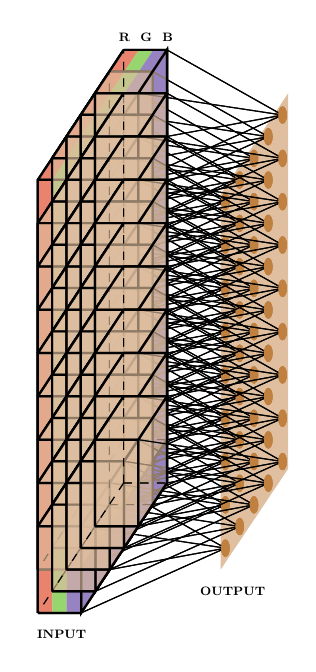
\begin{tikzpicture}[scale=.55, transform shape]
\def\h{10}
\def\w{2}
\def\d{3}
\coordinate (A) at (0,0);
\coordinate (B) at (0,\h);
\coordinate (C) at (\w,\h+\d);
\coordinate (D) at (\w,\d);

\coordinate (A01) at (0+0.3333,0);
\coordinate (B01) at (0+0.3333,\h);
\coordinate (C01) at (\w+0.3333,\h+\d);
\coordinate (D01) at (\w+0.3333,\d);

\coordinate (A02) at (0+0.6666,0);
\coordinate (B02) at (0+0.6666,\h);
\coordinate (C02) at (\w+0.6666,\h+\d);
\coordinate (D02) at (\w+0.6666,\d);

\coordinate (A1) at (0+1,0);
\coordinate (B1) at (0+1,\h);
\coordinate (C1) at (\w+1,\h+\d);
\coordinate (D1) at (\w+1,\d);


\node[] (input1) at (0.5,-0.5) {\footnotesize{ \textbf{INPUT}}};
\node[] (input1) at (2,13.3) {\footnotesize {\textbf{R}}};
\node[] (input1) at (2.5,13.3) {\footnotesize \textbf{G}};
\node[] (input1) at (3,13.3) {\footnotesize \textbf{B}};

\onslide<3->{
\node[] (input1) at (4.5,0.5) {\footnotesize \textbf{OUTPUT}};
}
\fill [draw=none, fill=red!90] (A) -- (B) -- (C) -- (C01) -- (B01) -- (A01) -- cycle; 
\fill [draw=none, fill=green!90] (A01) -- (B01) -- (C01) -- (C02) -- (B02) -- (A02) -- cycle;
\fill [draw=none, fill=blue!90] (A02) -- (B02) -- (C02) -- (C1) -- (D1) -- (A1) -- cycle;
\draw (A) -- (B) -- (C) (A) -- (A1) (B) -- (B1) (C) -- (C1) (A1) -- (B1) -- (C1) -- (D1) -- cycle;


\def\ha{2}
\def\wa{0.66}
\def\sa{1}
\def\wb{0.33}%shift
\def\sb{0.5}%shift
\def\hc{0.66}%next layer box
\def\wc{0.22}%next layer box size
\def\sc{0.33}
\def\xm{4} %distance of next box
\def\xmv{0.22}
\def\ymv{1}
\def\wid{1}


%layer1 feature map coordinates
\coordinate (A6) at (0+\xm+\xmv,0+\ymv);
\coordinate (B6) at (0+\xm+\xmv,\h-\sc);
\coordinate (C6) at (\w+\xm-\xmv,\h+\d-\ymv);
\coordinate (D6) at (\w+\xm-\xmv,\d+\sc);

\coordinate (A7) at (0+1+\xm+\xmv,0+\ymv);
\coordinate (B7) at (0+1+\xm+\xmv,\h-\sc);
\coordinate (C7) at (\w+1+\xm-\xmv,\h+\d-\ymv);
\coordinate (D7) at (\w+1+\xm-\xmv,\d+\sc);

\onslide<3->{
\fill [draw=none, fill=brown!50] (A6) -- (B6) -- (C6) --  (D6) -- cycle;	
}

\onslide<2>{
\def\xz{4}
\def\yz{4}
		\coordinate (A2) at (0+\xz*\wb,0+\yz+\xz*\sb);
		\coordinate (B2) at (0+\xz*\wb,\ha+\yz+\xz*\sb);
		\coordinate (C2) at (\wa+\xz*\wb,\ha+\sa+\yz+\xz*\sb);
		\coordinate (D2) at (\wa+\xz*\wb,\sa+\yz+\xz*\sb);
		
		\coordinate (A3) at (0+1+\xz*\wb,0+\yz+\xz*\sb);
		\coordinate (B3) at (0+1+\xz*\wb,\ha+\yz+\xz*\sb);
		\coordinate (C3) at (\wa+1+\xz*\wb,\ha+\sa+\yz+\xz*\sb);
		\coordinate (D3) at (\wa+1+\xz*\wb,\sa+\yz+\xz*\sb);
		
		
		\fill [draw=none, fill=brown!50, fill opacity=0.4] (A2) -- (B2) -- (C2) -- (C3) -- (D3) -- (A3) -- cycle; 
			
		\draw[thick] (A2) -- (B2) -- (C2) (A2) -- (A3) (B2) -- (B3) (C2) -- (C3) (A3) -- (B3) -- (C3) -- (D3) -- cycle;
		\draw[dashed] (D2) -- (A2) (D2) -- (C2) (D2) -- (D3);
		
		\node[] (input1) at (0+0.5+\xz*\wb,0+\yz+\xz*\sb-0.5) {\footnotesize{ \textbf{filter}}};
}		
		


\foreach \y [count=\yi from 0] in {8,7,6,5,4,3,2,1,0}{
	\foreach \x [count=\xi from \yi*5+3] in {0,1,2,3,4}{
		\ifthenelse{\xi<8}{
		\onslide<\xi>{	
		%kernel coordinates
		\coordinate (A2) at (0+\x*\wb,0+\y+\x*\sb);
		\coordinate (B2) at (0+\x*\wb,\ha+\y+\x*\sb);
		\coordinate (C2) at (\wa+\x*\wb,\ha+\sa+\y+\x*\sb);
		\coordinate (D2) at (\wa+\x*\wb,\sa+\y+\x*\sb);
		
		\coordinate (A3) at (0+1+\x*\wb,0+\y+\x*\sb);
		\coordinate (B3) at (0+1+\x*\wb,\ha+\y+\x*\sb);
		\coordinate (C3) at (\wa+1+\x*\wb,\ha+\sa+\y+\x*\sb);
		\coordinate (D3) at (\wa+1+\x*\wb,\sa+\y+\x*\sb);
		
		
		\fill [draw=none, fill=brown!50, fill opacity=0.4] (A2) -- (B2) -- (C2) -- (C3) -- (D3) -- (A3) -- cycle; 
			
		\draw[thick] (A2) -- (B2) -- (C2) (A2) -- (A3) (B2) -- (B3) (C2) -- (C3) (A3) -- (B3) -- (C3) -- (D3) -- cycle;
		\draw[dashed] (D2) -- (A2) (D2) -- (C2) (D2) -- (D3);

		%feature map 1, points
		\coordinate (A4) at (0+\x*\wb+\xm+\xmv,0+\y+\x*\sb+\ymv);
		\coordinate (B4) at (0+\x*\wb+\xm+\xmv,\hc+\y+\x*\sb+\ymv);
		\coordinate (C4) at (\wc+\x*\wb+\xm+\xmv,\hc+\sc+\y+\x*\sb+\ymv);
		\coordinate (D4) at (\wc+\x*\wb+\xm+\xmv,\sc+\y+\x*\sb+\ymv);
		\coordinate (ABCD4) at (\wc*0.5+\x*\wb+\xm+\xmv,\y+\x*\sb+\ymv+\hc*0.5+\sc*0.5);
		\draw (A3) -- (ABCD4);
		\draw (B3) -- (ABCD4);
		\draw (C3) -- (ABCD4);
		\draw (D3) -- (ABCD4);
		
		}
		\onslide<\xi->{
			\fill[brown] (ABCD4) ellipse (0.1 and 0.2);		
		}
		}{
		\ifthenelse{\xi > 7 \AND \xi < 40}{
		\onslide<8->{
			\coordinate (A4) at (0+\x*\wb+\xm+\xmv,0+\y+\x*\sb+\ymv);
			\coordinate (B4) at (0+\x*\wb+\xm+\xmv,\hc+\y+\x*\sb+\ymv);
			\coordinate (C4) at (\wc+\x*\wb+\xm+\xmv,\hc+\sc+\y+\x*\sb+\ymv);
			\coordinate (D4) at (\wc+\x*\wb+\xm+\xmv,\sc+\y+\x*\sb+\ymv);
			\coordinate (ABCD4) at (\wc*0.5+\x*\wb+\xm+\xmv,\y+\x*\sb+\ymv+\hc*0.5+\sc*0.5);		
			\fill[brown] (ABCD4) ellipse (0.1 and 0.2);
		}			
		}{
		\pgfmathparse{int(\xi-40+8)}
	 	\onslide<\pgfmathresult>{
	 	\coordinate (A2) at (0+\x*\wb,0+\y+\x*\sb);
		\coordinate (B2) at (0+\x*\wb,\ha+\y+\x*\sb);
		\coordinate (C2) at (\wa+\x*\wb,\ha+\sa+\y+\x*\sb);
		\coordinate (D2) at (\wa+\x*\wb,\sa+\y+\x*\sb);
		
		\coordinate (A3) at (0+1+\x*\wb,0+\y+\x*\sb);
		\coordinate (B3) at (0+1+\x*\wb,\ha+\y+\x*\sb);
		\coordinate (C3) at (\wa+1+\x*\wb,\ha+\sa+\y+\x*\sb);
		\coordinate (D3) at (\wa+1+\x*\wb,\sa+\y+\x*\sb);
		
		
		\fill [draw=none, fill=brown!50, fill opacity=0.4] (A2) -- (B2) -- (C2) -- (C3) -- (D3) -- (A3) -- cycle; 
			
		\draw[thick] (A2) -- (B2) -- (C2) (A2) -- (A3) (B2) -- (B3) (C2) -- (C3) (A3) -- (B3) -- (C3) -- (D3) -- cycle;
		\draw[dashed] (D2) -- (A2) (D2) -- (C2) (D2) -- (D3);

		%feature map 1, points
		\coordinate (A4) at (0+\x*\wb+\xm+\xmv,0+\y+\x*\sb+\ymv);
		\coordinate (B4) at (0+\x*\wb+\xm+\xmv,\hc+\y+\x*\sb+\ymv);
		\coordinate (C4) at (\wc+\x*\wb+\xm+\xmv,\hc+\sc+\y+\x*\sb+\ymv);
		\coordinate (D4) at (\wc+\x*\wb+\xm+\xmv,\sc+\y+\x*\sb+\ymv);
		\coordinate (ABCD4) at (\wc*0.5+\x*\wb+\xm+\xmv,\y+\x*\sb+\ymv+\hc*0.5+\sc*0.5);
		\draw (A3) -- (ABCD4);
		\draw (B3) -- (ABCD4);
		\draw (C3) -- (ABCD4);
		\draw (D3) -- (ABCD4);
		
		}
		\onslide<\pgfmathresult->{
			\fill[brown] (ABCD4) ellipse (0.1 and 0.2);		
		}		
		};		
		};
	}
}


\end{tikzpicture}
\end{center}
		\end{overlayarea}
		
		\column{0.6\textwidth}
		\begin{overlayarea}{\textwidth}{\textheight}
			\justifying
			\begin{itemize}
				\justifying
				\item<1-> What would a 3D filter look like?
				\item<2-> It will be 3D and we will refer to it as a volume
				\item<3-> Once again we will slide the volume over the 3D input and compute the convolution operation
				\item<15-> Note that in this lecture we will assume that the filter always extends to the depth of the image
				\item<16-> In effect, we are doing a 2D convolution operation on a 3D input (because the filter moves along the height and the width but not along the depth)
				\item<17-> As a result the output will be 2D (only width and height, no depth)
				\item<18-> Once again we can apply multiple filters to get multiple feature maps
			\end{itemize}
		\end{overlayarea}
	\end{columns}
\end{frame}
